
\documentclass[11pt,letterpaper]{article}

% Load some basic packages that are useful to have
% and that should be part of any LaTeX installation.
%
% be able to include figures
\usepackage{graphicx}
% get nice colors
\usepackage{xcolor}

% change default font to Palatino (looks nicer!)
\usepackage[latin1]{inputenc}
\usepackage{mathpazo}
\usepackage[T1]{fontenc}
% load some useful math symbols/fonts
\usepackage{latexsym,amsfonts,amsmath,amssymb}

% comfort package to easily set margins
\usepackage[top=1in, bottom=1in, left=1in, right=1in]{geometry}

% control some spacings
%
% spacing after a paragraph
\setlength{\parskip}{.15cm}
% indentation at the top of a new paragraph
\setlength{\parindent}{0.0cm}


\begin{document}

\begin{center}
\Large
Ay190 -- Worksheet 14\\
Anthony Alvarez\\
Date: February 27, 2014
\end{center}

\section{Advection Equation}

We will consider the advection equation.
$$ \frac{\partial u}{\partial t} + u \frac{\partial u}{\partial x} = 0$$

We use it to advect a Gaussian
$$ \Psi_0 = \Psi(x,t=0) = \frac18 \sin(2\pi x/L)$$.
Where $L = 100$ a $[0,100]$ domain. 

\subsection{Shock Develops}

As you can see in myadvect.py I have implemented the upsind scheme.

We notice that the section of the sin wave with $u>0$ moves to the right,
positive $x$. While the section of the sin wave with $u<0$ moves to the left,
negative $x$. This results in the shock at $x = 0$ at around $t \approx 140$

You can see the shock develop in figure ~\ref{fig:1} at  $t = 121$, devolop 
defined features by $t=145$ ~ref{fig:2} and be
completely formed in figure ~\ref{fig:3} at $t=200$

\begin{figure}[bth]
\centering
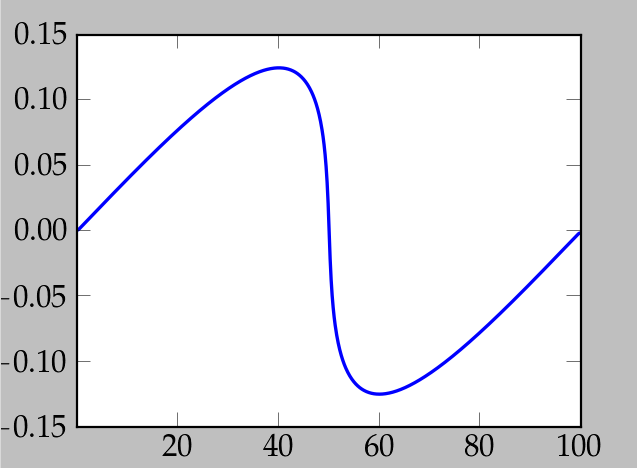
\includegraphics[width=0.5\textwidth]{t=121.png}
\caption{Begining of shock development from upwind scheme evolution of Burger's
equation at $t=121$.}
\label{fig:1}
\end{figure}

\begin{figure}[bth]
\centering
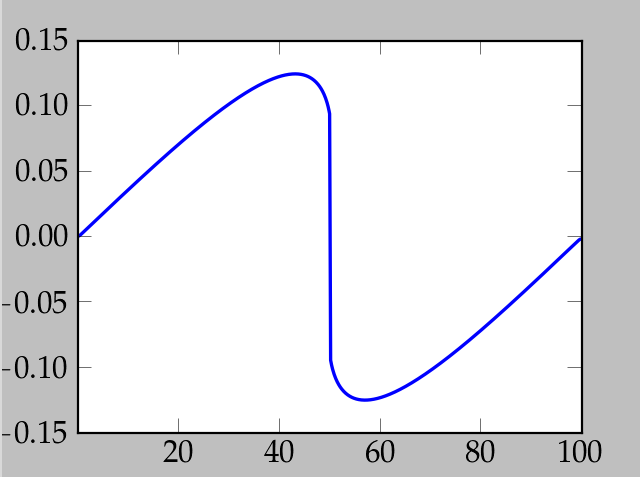
\includegraphics[width=0.5\textwidth]{t=145.png}
\caption{Strong shock development from upwind scheme evolution of Burger's
equation at $t=145$.}
\label{fig:2}
\end{figure}

\begin{figure}[bth]
\centering
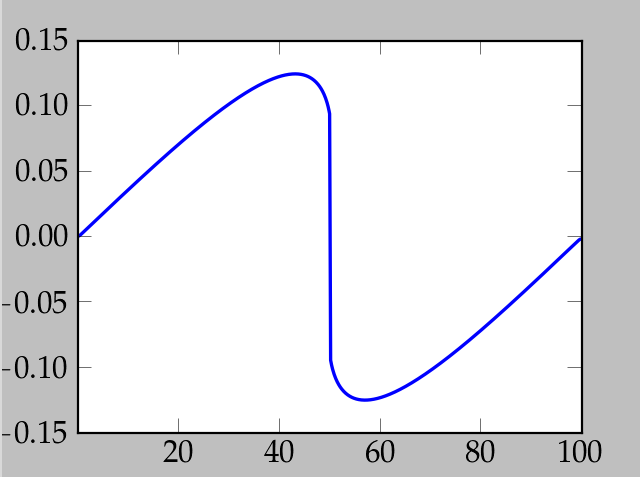
\includegraphics[width=0.5\textwidth]{t=145.png}
\caption{Complete shock development from upwind scheme evolution of Burger's
equation at $t=200$.}
\label{fig:3}
\end{figure}


\end{document}




